% IEEE Conference Template: https://www.overleaf.com/latex/templates/ieee-conference-template/grfzhhncsfqn
\documentclass[conference]{IEEEtran}
\usepackage{cite}
\usepackage{amsmath,amssymb}
\usepackage{graphicx}
\usepackage{booktabs}
\usepackage[hidelinks]{hyperref}
% Generated by eval.plot_audited_comparison.
\newcommand{\AuditDelay}{60.54}
\newcommand{\AuditLoss}{24.88}
\newcommand{\AuditGoodput}{6.62}
\newcommand{\AuditStaticReduction}{25.15}
\newcommand{\AuditCadenceReduction}{15.65}
\newcommand{\AuditNeuralReduction}{1.22}
\newcommand{\AuditNeuralLossDelta}{0.33}
\newcommand{\AuditNeuralGoodputDelta}{-0.027}
\newcommand{\AuditNeuralHolm}{0.0014}
\newcommand{\AuditDPPDelta}{0.12}
\newcommand{\AuditDPPHolm}{0.0745}
\newcommand{\AuditNoLoRADelta}{0.48}
\newcommand{\AuditNoLoRAHolm}{0.0054}
\newcommand{\AuditCritiqueCalls}{432}
\newcommand{\AuditCritiqueRevisions}{0}
\newcommand{\AuditMemoryPrompts}{420}
\newcommand{\AuditSpecialistBallots}{360}
\newcommand{\AuditGovernorCalls}{72}
\newcommand{\AuditPriorChanges}{2920}

% Generated by plot_manuscript.py
\newcommand{\AuditManuscriptRows}{%
S0 Static & 80.88 & 26.00 & 6.509 \\
S1 Base LM & 61.30 & 24.55 & 6.648 \\
S2 Base LM + critique & 61.34 & 24.55 & 6.648 \\
S3 Direct LoRA & 79.40 & 25.94 & 6.515 \\
S4 Agentic at 5 s & 71.77 & 25.33 & 6.574 \\
\textbf{S5 SELF-X} & 60.54 & 24.88 & 6.621 \\
Capacity threshold & 69.04 & 25.22 & 6.584 \\
Least loaded & 70.85 & 25.29 & 6.577 \\
Tabular Q & 71.52 & 25.39 & 6.567 \\
DQN & 61.29 & 24.55 & 6.648 \\
Two-agent IQL & 61.29 & 24.55 & 6.648 \\
DPP only & 60.42 & 24.57 & 6.646 \\
S5 without LoRA & 60.07 & 24.56 & 6.647 \\
S5 without governor & 60.41 & 24.58 & 6.644 \\
}

% Generated by revision_analysis.py
\newcommand{\AuditInteraction}{0.49}
\newcommand{\AuditUndeliveredDelta}{0.33}
\newcommand{\AuditBacklogFull}{0.17}
\newcommand{\AuditBacklogDQN}{0.17}
\newcommand{\AuditGoodputThree}{6.621}
\newcommand{\AuditBootCadence}{[-13.28, -9.15]}
\newcommand{\AuditBootNeural}{[-0.89, -0.60]}
\newcommand{\AuditBootDPP}{[0.04, 0.19]}
\newcommand{\AuditMeterShare}{0.32}
\newcommand{\AuditCadenceSteady}{-5.79}
\newcommand{\AuditCadenceFlash}{-1.66}
\newcommand{\AuditCadenceVolatile}{-26.25}
\newcommand{\AuditPairedRows}{%
S0 & -20.342 & [-27.506, -13.179] & 0.0025 & 0.0102 \\
S1 & -0.755 & [-0.964, -0.546] & 0.0001 & 0.0014 \\
S2 & -0.802 & [-0.997, -0.607] & 0.0001 & 0.0012 \\
S3 & -18.857 & [-26.011, -11.703] & 0.0032 & 0.0102 \\
S4 & -11.232 & [-14.566, -7.899] & 0.0006 & 0.0048 \\
TH & -8.503 & [-10.704, -6.301] & 0.0002 & 0.0014 \\
LL & -10.311 & [-13.672, -6.950] & 0.0012 & 0.0070 \\
TQ & -10.984 & [-14.111, -7.857] & 0.0012 & 0.0070 \\
DQN & -0.749 & [-0.957, -0.540] & 0.0001 & 0.0014 \\
IQL & -0.749 & [-0.957, -0.540] & 0.0001 & 0.0014 \\
DPP & +0.121 & [0.010, 0.232] & 0.0372 & 0.0745 \\
NL & +0.476 & [0.339, 0.613] & 0.0008 & 0.0054 \\
NG & +0.136 & [0.001, 0.271] & 0.0488 & 0.0745 \\
}

% Generated by plot_expanded_paper.py
\newcommand{\ExpandedProfileRows}{%
Steady bursts & S0 & 93.11 & 31.73 & 5.857 \\
 & S4 & 87.08 & 31.16 & 5.909 \\
 & S5 & 81.29 & 30.82 & 5.941 \\
 & DPP & 81.34 & 30.82 & 5.941 \\
 & DQN/IQL & 81.29 & 30.81 & 5.941 \\
\addlinespace
Flash crowd & S0 & 51.60 & 34.80 & 5.112 \\
 & S4 & 50.94 & 34.93 & 5.104 \\
 & S5 & 49.28 & 35.40 & 5.070 \\
 & DPP & 49.30 & 34.78 & 5.114 \\
 & DQN/IQL & 50.01 & 34.78 & 5.114 \\
\addlinespace
Volatile & S0 & 97.94 & 11.48 & 8.557 \\
 & S4 & 77.30 & 9.92 & 8.708 \\
 & S5 & 51.05 & 8.43 & 8.852 \\
 & DPP & 50.62 & 8.11 & 8.883 \\
 & DQN/IQL & 52.57 & 8.06 & 8.888 \\
}

\newcounter{selfxalgorithm}
\begin{document}

\title{SELF-X: Evaluating Language Model Assistance for Flow Control in Software-Defined Networks}
\author{%
\IEEEauthorblockN{Ganesh Reddy J\IEEEauthorrefmark{1},
M Jagadeswar\IEEEauthorrefmark{1},
Harsh Raj\IEEEauthorrefmark{1},\\
C Sai Aravind\IEEEauthorrefmark{1},
Koushik C\IEEEauthorrefmark{2},
Dhruv R Katti\IEEEauthorrefmark{3}}
\IEEEauthorblockA{%
\IEEEauthorrefmark{1}Dept.\ of Data Science and Artificial Intelligence\\
\IEEEauthorrefmark{2}Dept.\ of Computer Science and Engineering\\
\IEEEauthorrefmark{3}Dept.\ of Electronics and Communication Engineering\\
\textit{Indian Institute of Information Technology Dharwad}, Dharwad, Karnataka, India\\
Team SDN\_07, EC466 Software Defined Networks\\
\{23bds024, 23bds033, 23bds076, 23bds075, 23bcs073, 23bec015\}@iiitdwd.ac.in}}
\maketitle

\begin{abstract}
We evaluate whether language model advice improves an analytic controller for congestion management in software-defined networks. SELF-X combines a drift-plus-penalty controller, a frozen low-rank adapter that suggests flow actions, and a slower language model that adjusts objective weights. Fourteen configurations share a finite-buffer fluid datapath and twelve paired synthetic traffic traces. The full controller lowers mean delay by \AuditStaticReduction{} percent relative to static forwarding and by \AuditCadenceReduction{} percent relative to the same stack with a five-second decision cadence. Relative to a trained deep Q-network, it lowers mean delay by \AuditNeuralReduction{} percent while losing \AuditNeuralLossDelta{} percentage points more traffic. The full stack is \AuditDPPDelta{} ms slower than fast drift-plus-penalty control alone; that difference does not survive multiplicity correction. Adding the adapter preference to the governed controller increases delay by \AuditNoLoRADelta{} ms. The governor repeats one adjustment throughout the test set, and critique never revises an action. These results support faster analytic actuation in this simulator, with no demonstrated incremental delay benefit from the combined language model layers.
\end{abstract}
\begin{IEEEkeywords}
software-defined networking, congestion management, drift-plus-penalty, language models, reinforcement learning
\end{IEEEkeywords}

\section{Introduction}
A software-defined network (SDN) separates forwarding from a programmable control plane~\cite{mckeown2008openflow}. Consider a bottleneck carrying background traffic and bursts of bulk traffic. A controller can move the bulk traffic to another path or meter it at ingress. Rerouting consumes capacity on the alternate path and can increase propagation delay; metering can reduce queues by discarding traffic before it enters the network. At a constant arrival rate \(a_i>c_i\), an empty buffer fills in \(B/(a_i-c_i)\) seconds: for example, 200~ms for 20~Mbps of arrivals, 10~Mbps of service, and a 2~Mbit buffer. Delay alone cannot establish that an intervention helped.

SELF-X separates the time at which it applies forwarding decisions from the times at which it requests model advice. We ask three questions: How much does the actuation cadence matter when the rest of the stack stays fixed? Do the action prior and objective governor add value to fast analytic control? How does the resulting delay compare with trained value-based controllers when loss and goodput are also counted?

We contribute a constrained implementation on a shared finite-buffer model, a paired experiment with fourteen reference and ablation configurations, and execution traces that distinguish model output, proposed actions, and applied actions. The experiment concerns a single simulated topology and does not test production OpenFlow timing.

\section{Related Work}
OpenFlow exposes programmatic forwarding~\cite{mckeown2008openflow}, and equal-cost multipath routing describes how to select among paths for forwarding~\cite{hopps2000ecmp}. Our least-loaded baseline is a queue-based two-path heuristic. We use the drift-plus-penalty (DPP) principle from stochastic network optimization~\cite{neely2010stochastic} as the basis for a finite-horizon decision score. The experiment does not establish a Lyapunov stability theorem.

Deep reinforcement learning has been applied to network control~\cite{xu2018experience}; multi-agent reinforcement learning has also been studied for SDN congestion management~\cite{boussaoud2025marl}. Our deep Q-network (DQN) follows replay and target-network methods~\cite{mnih2015human}, while the independent Q-learning (IQL) comparator is a project-specific two-agent design with shared observations and rewards. Neither is a reproduction of a published SDN system.

Prior work applies language model agents to dynamic SDN management~\cite{araujo2024agentic}, adapts language models to networking tasks~\cite{wu2024netllm}, and studies slow governance for SDN and IoT defense~\cite{jamshidi2026governance} and reflection for adaptive radio access network slicing~\cite{li2026redsi}. SELF-X instead studies routing and metering for a bulk aggregate. Its critique arm is motivated by verbal reflection~\cite{shinn2023reflexion}; the action prior uses low-rank adaptation (LoRA)~\cite{hu2022lora} on SmolLM2~\cite{allal2025smollm2}. We test these mechanisms separately from the fast loop rather than infer their value from the full system's comparison with static forwarding.

\section{Problem Scenario and System Model}
The controller observes primary background demand \(m\), bulk demand \(e\) (both Mbps), and current path backlogs \(q_i\) (Mbit) at each 100~ms slot. Both paths have capacity \(c_i=10\)~Mbps and a \(B=2\)~Mbit buffer; their propagation delays \(d_i\) are 2 and 12~ms. Background traffic stays on primary. The bulk aggregate can stay on primary (\(P\)), move intact to alternate (\(A\)), or be metered on primary (\(M\)). The model has no unrelated traffic on alternate, no per-flow splitting, and no transport response to loss.

For a slot of length \(\tau=0.1\)~s, let \(\tilde e=\min(e,r)\) for a meter ceiling \(r\) and \(\tilde e=e\) otherwise. The admitted path rates \(a_i\) are \((m,\tilde e)\) under \(A\) and \((m+\tilde e,0)\) otherwise. With \([z]_+=\max(0,z)\) and \([z]_0^B=\min(B,[z]_+)\), the simulator uses
\begin{align}
x_i &= q_i+(a_i-c_i)\tau, \quad q_i'=[x_i]_0^B, \\
o_i &= [x_i-B]_+, \quad s_i=q_i+a_i\tau-q_i'-o_i,\\
D_m &= (e-\tilde e)\tau, \quad O=(m+e)\tau .
\end{align}
Here \(s_i,o_i,D_m,O\) are served, overflowed, metered and offered volumes. Backlog carries forward even when the selected path changes. Including metered bits yields \(\sum_i q_i+O=\sum_i(q_i'+s_i+o_i)+D_m\). The code checks the equivalent conservation relation after ingress metering.

Let \(\bar q_i=\tau^{-1}\int_0^\tau[q_i+(a_i-c_i)u]_0^B\,du\). The clipped integral captures filling or draining within a slot. If a queue hits 0 or \(B\), the integral combines a trapezoid up to the hit time with a constant segment at the boundary. With \(S=\sum_i s_i\) and \(L=\sum_i o_i+D_m\), its slot metrics are goodput \(G=S/\tau\), loss fraction \(\ell=L/O\), and delay
\begin{equation}
D=\frac{\sum_i s_i(d_i+1000\bar q_i/c_i)}{S}.
\label{eq:delay}
\end{equation}
For zero service the code uses primary propagation delay; loss is zero for zero offered volume. The queue term in~\eqref{eq:delay} represents virtual waiting time at the path's service rate. It is a fluid proxy. In window \(w\), the delay is \(\sum_{t\in w} S_tD_t/\sum_{t\in w}S_t\), with the same fallback when no traffic is served.

\section{Controller and Mathematical Formulation}
\subsection{Feasible action set and fast optimizer}
The shared guard allows \(P\) unconditionally, \(A\) when \(e\leq0.9c_2\), and \(M\) when \(e>0\), \(r\geq0.512\)~Mbps, and \(\max(0,1-r/e)\leq0.20\). Outside this set, a proposed action resolves to \(P\). The DPP, direct-model, and neural arms construct a meter locally as
\begin{equation}
r=\frac{\lfloor 1000\min\{\max(0.512,9-m),\,
                          \max(0.85e,0.512)\}\rfloor}{1000}.
\label{eq:meter}
\end{equation}
The threshold and tabular arms propose \(r=\lfloor1000\max(0.5,9-m)\rfloor/1000\)~Mbps. The guard can reject either meter rule when the cap would discard more than 20\% of bulk demand, or when the baseline's 0.5~Mbps floor violates the guard's 0.512~Mbps minimum.

At a decision, the optimizer knows the exact rates and backlogs for the current slot and has the simulator's transition model; it does not see future demand. The fast neural baselines see the same current telemetry but do not evaluate counterfactual transitions with this model. For each feasible action \(u\), the fast controller predicts \(D,\ell,G\) from the same transition as the datapath and scores
\begin{align}
J(u) &= \sum_i q_i(a_i(u)-c_i)+V\,C(u), \label{eq:score}\\
C(u) &= w_d D/50+w_\ell\ell-w_gG/10
        +w_E E(u)+w_R R(u).
\end{align}
The queue term is a rate-form drift surrogate in Mbit\({}^2\)/s. Multiplication by \(\tau\) gives the linear term in the unclipped quadratic drift; the code scores the rate form shown, with \(V\) on the same scale. Physical buffer clipping bounds the queue size, but supplies no stability or loss guarantee. The initial \(V=8\) and \((w_d,w_\ell,w_g,w_E,w_R)=(0.25,0.25,0.25,0.15,0.10)\). The dimensionless energy proxies \(E(P),E(A),E(M)\) are \(0.35,1.70,0.35\) and resource proxies \(R(P),R(A),R(M)\) are \(0,0.55,0.40\). These are configured costs, not measured energy or resource use. The optimizer enumerates up to three actions. A feasible model preference \(h\) changes the selection to \(\arg\min_u[\operatorname{round}(J(u),6)+0.20\,\mathbf{1}(u\ne h)]\); otherwise it uses the unrounded DPP minimum. The optimizer rechecks preference feasibility at each decision. If \(h\) is infeasible, it ignores the preference rather than replacing it with \(P\). Ties follow the order \(P,A,M\). The learning reward in Sec.~\ref{sec:design} is separate.

\subsection{Slow advice and execution order}
Every 5~s the adapter and the direct base-model arms query the same action prompt. It reports projected primary and alternate loads from demand rounded to 0.5~Mbps, capacity, and overload and reroute-feasibility flags. It omits queues and prior outcomes. The largest logit among the three action tokens selects the suggestion. The preference first becomes available at 0.4~s, so S5 uses unrounded DPP in the first four slots.

Every 30~s the same bare model evaluates five specialist prompts (flow sizing, routing, congestion, safety and service) as one batch. Each receives the current background and bulk rates rounded to integer Mbps and the two queues rounded to integer Mbit. The orchestrator receives this snapshot and the ballots, without past outcomes or current objective weights. It selects \((\Delta V,\Delta\mathbf{w})\): a decrement of 2 and increment \(\mathbf{b}\), no change, or the opposite. Here \(\mathbf{b}=(0.06,0.06,0.00,-0.07,-0.05)\). After eight slots, on a nonzero update,
\begin{align}
V'&=\min(32,\max(0.5,V+\Delta V)),\\
z_j&=\max(0,w_j+\Delta w_j),\quad w'_j=z_j/\sum_k z_k .
\end{align}
The governor cannot modify the action menu. The initial objective stays in force until the first update at 0.8~s.

In each slot SELF-X reads demand and queues, schedules any due model requests, incorporates advice whose simulated ready time has arrived, minimizes~\eqref{eq:score} with the optional preference, and checks the proposal before advancing the datapath. The fast loop continues on the previous parameters while advice is pending. The model executes actual local forward passes for uncached requests. All model stages, including cache hits, are charged 0.4~s per sequential stage in simulated time. The evaluation does not measure model or switch latency.

\begin{figure*}[t]
\centering
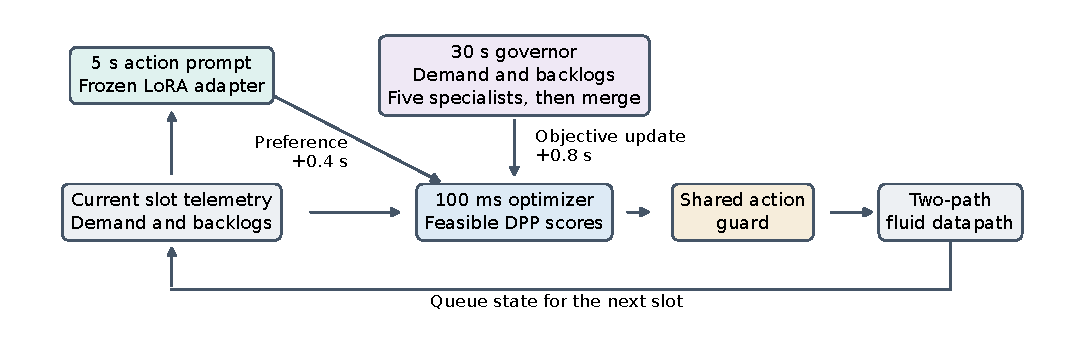
\includegraphics[width=.95\textwidth]{comparison/paper_architecture.pdf}
\caption{The implemented S5 control path. The adapter supplies a preference and the governor updates the objective. The optimizer proposes an action, the guard selects the effective action, and the datapath returns the next slot's queues. The two advice delays are simulation parameters.}
\label{fig:architecture}
\end{figure*}

\section{SELF-X Execution}
\label{sec:execution}
Figure~\ref{fig:architecture} shows how S5 uses two types of model advice. The 5~s adapter suggests an action kind. The 30~s governor changes the weight and scale of the operating penalty. The 100~ms loop consumes both and reevaluates the feasible actions as load and backlogs change. The guard remains active even between optimizer decisions.

\subsection{Control scheduler}
Algorithm~\ref{alg:scheduler} gives the scheduling order for S4 and S5. The 5~s and 30~s periods correspond to 50 and 300 slots. The 0.4 and 0.8~s offsets correspond to four and eight slots. At the beginning of an episode, the fast loop starts with the configured objective and no active preference. This ordering matters in S4 because the decision at a window boundary occurs before either new model response is due.

\begin{table}[t]
\refstepcounter{selfxalgorithm}
\label{alg:scheduler}
\noindent\textbf{Algorithm \theselfxalgorithm.} Scheduling and actuation in S4 and S5\par\smallskip
\small
\begin{tabular}{@{}r@{\quad}p{.86\columnwidth}@{}}
\toprule
 & Initialize queues to zero, preference to unset, and proposal to \(P\).\\
1 & Read slot demand and backlogs.\\
2 & Every 300 slots, request the governor update using this slot's demand and backlogs and schedule it for slot \(t+8\).\\
3 & Every 50 slots, request the adapter token using this slot's demand and schedule it for slot \(t+4\).\\
4 & Apply any due update to \(V,\mathbf{w}\) and activate any due preference.\\
5 & In S5, or at a 50-slot boundary in S4, replace the proposal with the result of Algorithm~\ref{alg:action}.\\
6 & Check the held proposal against current demand. Use \(P\) for this slot if the guard rejects it.\\
7 & Advance the fluid datapath, carry over its queues, and record the outcome. Repeat at the next slot.\\
\bottomrule
\end{tabular}
\end{table}

\begin{table}[t]
\refstepcounter{selfxalgorithm}
\label{alg:action}
\noindent\textbf{Algorithm \theselfxalgorithm.} Computing the DPP proposal\par\smallskip
\small
\begin{tabular}{@{}r@{\quad}p{.86\columnwidth}@{}}
\toprule
1 & Construct \(P,A,M\), computing the meter ceiling for \(M\) using~\eqref{eq:meter}.\\
2 & Evaluate the shared guard and keep feasible candidates in the order \(P,A,M\).\\
3 & Predict one slot's outcome and compute \(J(u)\) for each retained candidate using~\eqref{eq:score}.\\
4 & If the active preference \(h\) is feasible, minimize the rounded score with a \(0.20\) penalty on \(u\ne h\). Otherwise minimize the unrounded score.\\
5 & Return the first minimizer with its meter ceiling, if any.\\
\bottomrule
\end{tabular}
\end{table}

\subsection{Model execution and direct control}
The adapter uses the pinned SmolLM2-135M-Instruct checkpoint. The implementation caches repeated prompts and still schedules each response at its modeled ready time. The governor uses a single batched specialist pass followed by an orchestrator pass on the base model. Each pass chooses from three tokens. The orchestrator's token identifies a fixed update to \(V\) and the weights.

S1 and S3 use the predicted action directly at the ready time. For S2, a second prompt sees the first proposal, the rounded current state, and up to three completed window outcomes. The critique token replaces the first token at its ready time. At each window end, S2 records the last applied action and realized window reward. These tuples provide context for later critique. The adapter used in S3 through S5 is already trained when evaluation begins.


\section{Baselines and Experimental Setup}\label{sec:design}
\subsection{Configuration design}
Table~\ref{tab:controllers} defines the fourteen arms. S4 holds each proposal and its numeric meter ceiling until the next 5~s decision. Its LoRA and governor advice arrive at the same times as in S5 but are consumed only at the next decision, after an additional 4.6 and 4.2~s, respectively. All slower controllers hold their proposal parameters between updates. A guard veto affects only the current slot; the held proposal is reconsidered in the next slot. S1 and S3 propose a direct action every 5~s, applied after the 0.4~s model delay. S2 adds one delayed critique pass prompted with the proposal and up to three prior realized action--reward pairs. It applies the final action after 0.8~s. This measures critique with its extra modeled latency; there is no latency-matched S1 control. The history records the final effective action and the realized reward of each completed window. Governance does not write to this history, and critique does not retrain model weights.

\begin{table}[t]
\centering
\caption{Configurations and Decision Cadences}
\label{tab:controllers}
\footnotesize
\begin{tabular}{@{}llr@{}}
\toprule
ID & Controller & Cadence \\
\midrule
S0 & Static & Fixed \\
S1 & Base LM & 5 s \\
S2 & Base LM plus critique & 5 s \\
S3 & Direct LoRA & 5 s \\
S4 & Agentic at 5 s (full stack) & 5 s \\
S5 & SELF-X (full stack) & 100 ms \\
TH & Capacity threshold & 5 s \\
LL & Least loaded & 5 s \\
TQ & Tabular Q (online) & 5 s \\
DQN & DQN (frozen) & 100 ms \\
IQL & Two-agent IQL (frozen) & 100 ms \\
DPP & DPP only & 100 ms \\
NL & S5 without LoRA & 100 ms \\
NG & S5 without governor & 100 ms \\
\bottomrule
\end{tabular}
\end{table}

The capacity heuristic leaves demand on primary up to 85\% of capacity, then prefers rerouting if the alternate queue is below 0.25~Mbit and projected utilization is at most 90\%; it otherwise proposes a meter. Least loaded considers only \(P,A\); it prefers alternate when its queue is shorter and bulk demand fits its nominal capacity. At \(m=3\)~Mbps, the common model/DPP/neural meter cap is at most 6~Mbps and the guard rejects it for \(e>7.5\)~Mbps. Tabular Q-learning explores from a cold start within each test episode; it floors \(m/1.5,e/2,2q_1,2q_2\), caps the resulting integers at \(4,6,4,4\), and uses learning rate 0.25, discount 0.90, and initial exploration 0.20 (decay 0.995 per update, floor 0.02). This is an online cold-start reference. The trained neural policies provide the separate offline-trained comparison.

DQN and both IQL agents see \((m/10,e/20,q_1/2,q_2/2)\) plus a one-hot previous applied action. The IQL route agent votes primary or alternate; the meter agent votes off or on. Alternate wins regardless of the meter vote. Otherwise an on vote proposes \(M\), and off proposes \(P\). Both agents store their own vote and the common realized reward. Each network has two 64-unit ReLU layers, its own 20,000-transition replay buffer and Adam step size 0.001. Training uses minibatches of 64, a Huber loss, discount 0.97, a gradient step every eight slots once the buffer is ready, and a target copy every 100 steps. Neural exploration uses \(\max(0.05,1-k/18000)\) at global training slot \(k\); evaluation is greedy and frozen. All three networks completed 2,692 updates and 26 target synchronizations. Their reward for a training slot is \(G/10-D/50-1.5\ell-2.5I\), where \(I\) is one when the effective rule changes and zero otherwise. The window version used for tabular training and critique uses window metrics and subtracts 0.05 per rule change. The learning reward gives loss more relative weight than the initial DPP penalty, charges switching explicitly, and omits the energy and resource proxies. The trade-offs therefore compare configured policies, not algorithms optimizing a common objective.

\subsection{Traffic, measurement, and inference}
Synthetic background demand is fixed per trace at 3~Mbps with up to 0.1~Mbps of seeded jitter. The steady-bursty profile has exponentially spaced bursts (15~s mean, 8--15~Mbps, 4--10~s). The flash-crowd generator checks the current event clock against the 30--70\% interval before sampling the next spacing. Inside it uses a 4~s exponential mean, 10--15~Mbps and 4--8~s duration; outside it uses 18~s, 4--8~Mbps and 3~s. Volatile traffic uses \(\max(1,\operatorname{round}(6+4\sin(t/5)+2\cos(t/2)+\eta,2))\)~Mbps at 0.5~s steps, with \(\eta\) uniform on \([-1.5,2.5]\). Concurrent bulk events are summed into the one steerable aggregate. The seed modulo three selects the profile. DQN and IQL train on seeds 1000--1017 for 120~s each and are tested on seeds 2100--2111 for 180~s each, four per profile. Network initialization uses 3928 for DQN and 3928 and 3929 for IQL. The frozen LoRA checkpoint comes from 150 synthetic replay episodes. Its metadata records 24 distinct states: 13 for training and 11 for the promotion gate, with gate seeds 1903--1904. Its offline grid steps for background, bulk and queue are 0.5~Mbps, 1.0~Mbps and 0.5~Mbit. The label rule favors the action with the highest mean realized reward in a \(3\times3\) neighborhood, weighting the exact state twice. Training used rank 8 and 60 steps. The gate seeds are distinct from the test seeds. Code, checkpoint, training metadata, and the pinned model identity are in the artifact.

The test has \(14\times12=168\) runs and \(168\times1800=302{,}400\) simulated slots. All arms start with empty queues and primary forwarding. Each paired seed has identical offered-slot traffic across all arms, verified by a fingerprint. A seed's mean delay is the arithmetic mean of its 36 five-second windows, with slot delays within each window weighted by served volume. This gives each time window equal influence rather than giving higher-volume windows greater weight. Seed loss is total overflow and metered volume divided by total offered volume; goodput is total served divided by 180~s. Traffic still queued at the end is neither served nor counted as loss. By volume balance, mean terminal backlog is \AuditBacklogFull~Mbit for S5 and \AuditBacklogDQN~Mbit for DQN/IQL. Counting terminal backlog as undelivered volume leaves their gap at \AuditUndeliveredDelta{} percentage points. Episode-wide volume-weighted delays and per-seed ending backlogs are included in the artifact. The main estimand is the mean of the three profile means of paired seed delay differences (S5 minus comparator). If profile \(j\) has sample variance \(s_j^2\) and \(n_j=4\) paired differences, its contribution to the estimated variance is \(s_j^2/(9n_j)\). We use a Welch--Satterthwaite \(t\) approximation for pointwise 95\% intervals and adjust two-sided delay tests across thirteen comparisons using Holm's procedure~\cite{holm1979simple}. Both neural arms count in the original thirteen-test family. Counting their identical realized delays once leaves the 5\% decisions unchanged. Loss and goodput are descriptive secondary outcomes. The independent unit of analysis is a seed, not a window or slot. As a sensitivity check, we also resample paired traces within each profile (20,000 draws, seed 466) and take pointwise percentile intervals. With only four traces per profile, this bootstrap is descriptive; it does not replace the Holm-adjusted tests.

\section{Results and Performance Analysis}
\begin{table}[t]
\centering
\caption{Mean Performance on Twelve Paired Synthetic Traces}
\label{tab:results}
\footnotesize
\setlength{\tabcolsep}{4.5pt}
\begin{tabular}{@{}lrrr@{}}
\toprule
Controller & Delay (ms) & Loss (\%) & Goodput (Mbps) \\
\midrule
\AuditManuscriptRows
\bottomrule
\end{tabular}
\end{table}

\begin{figure}[t]
\centering
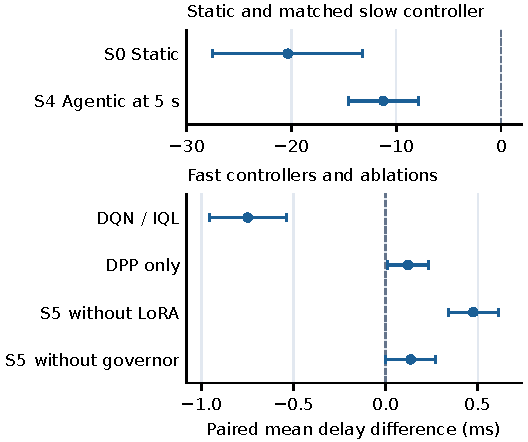
\includegraphics[width=\columnwidth]{comparison/paper_delay_effects.pdf}
\caption{Mean paired delay difference for S5 minus selected comparators. Negative values favor S5 on delay. Bars are pointwise 95\% confidence intervals; the comparison tests use Holm adjustment. The plotted scale changes between panels.}
\label{fig:effects}
\end{figure}

\begin{figure}[t]
\centering
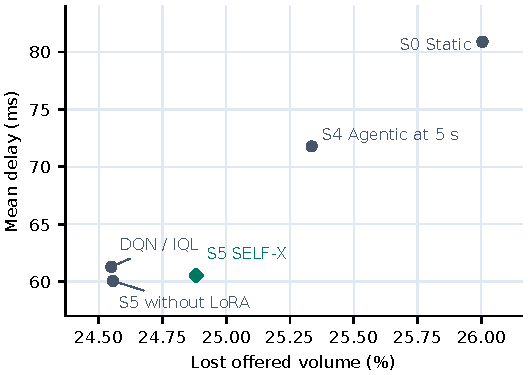
\includegraphics[width=\columnwidth]{comparison/paper_delay_loss.pdf}
\caption{Loss and delay across test seeds for selected configurations. Each marker is a mean over the twelve seeds. Down and left is preferable. The five markers are S0, S4, S5, S5 without LoRA, and the coincident DQN/IQL point.}
\label{fig:tradeoff}
\end{figure}

\subsection{Cadence and the static comparison}
S5 averages \AuditDelay~ms, \AuditLoss\% loss, and \AuditGoodputThree~Mbps (Table~\ref{tab:results}). It reduces mean delay by \AuditStaticReduction\% versus static forwarding and by \AuditCadenceReduction\% versus S4. Figure~\ref{fig:effects} gives the paired effects. The S4 comparison changes the DPP decision cadence while retaining the other two schedules. The paired delay changes are \(\AuditCadenceSteady\), \(\AuditCadenceFlash\), and \(\AuditCadenceVolatile\)~ms for steady bursts, flash crowds and volatile traffic, respectively. The trace bootstrap interval for the overall S5--S4 difference is \(\AuditBootCadence\)~ms.

\subsection{Comparison with trained controllers}
S5 lowers delay by \AuditNeuralReduction\% versus each neural baseline (paired difference \(-0.75\)~ms, pointwise 95\% CI \([-0.96,-0.54]\)~ms; adjusted \(p=\AuditNeuralHolm\)). It also loses \AuditNeuralLossDelta{} percentage points more offered traffic and changes goodput by \(\AuditNeuralGoodputDelta\)~Mbps (Fig.~\ref{fig:tradeoff}). Both neural baselines made different raw proposals but produced identical applied per-slot action and meter sequences, verified using action hashes. Instrumented replay found 891 different proposals in 21,600 slots (4.13\%); every disagreement involved a guard veto and both effective actions were primary forwarding. Neither neural arm applied metering. S1 and S2 also applied no meters, with the same offered-volume loss and goodput as the neural arms but slightly different delay. Their held proposals are still filtered every slot. S5 averages 130.6 effective rule changes per 180~s trace, versus 15.1 for S4, 106.2 for DPP alone, and 24.8 for DQN and IQL. These are simulator rule-state changes, including meter-rate changes. Metering accounts for \AuditMeterShare\% of offered volume in S5 and zero in DQN and IQL. Buffer overflow accounts for the rest of the observed loss. We do not estimate an unavoidable loss floor: arrivals above total instantaneous capacity can be absorbed by available queue space.

\subsection{Incremental effect of the model layers}
S5 is \AuditDPPDelta~ms slower than DPP alone (adjusted \(p=\AuditDPPHolm\)); Table~\ref{tab:paired} shows all paired tests. Effects use unrounded seed results, so a difference may not equal the subtraction of rounded table means. Trace bootstrap intervals are \(\AuditBootNeural\)~ms versus DQN/IQL and \(\AuditBootDPP\)~ms versus DPP alone. These pointwise intervals do not provide familywise significance. Removing LoRA from S5 improves delay by \AuditNoLoRADelta~ms (adjusted \(p=\AuditNoLoRAHolm\)). With no governor, adding LoRA changes mean delay by \(-0.015\)~ms relative to DPP; with the governor it increases delay by \AuditNoLoRADelta~ms. The descriptive difference of these LoRA effects is \AuditInteraction~ms. The repeated governor update reduces \(V\) from 8 to 0.5 by 90.8~s (updates at 0.8, 30.8, 60.8, and 90.8~s) while the LoRA margin stays at 0.20. This makes the preference larger relative to the penalty term, but the ablations do not isolate the change in \(V\) from the simultaneous reweighting or from differences in visited states. The prior changes \AuditPriorChanges{} of 21,600 optimizer choices relative to the DPP decision at the same visited state and objective. The governor produces \AuditGovernorCalls{} decisions and \AuditSpecialistBallots{} ballots in S5; every ballot and merge chooses the same queue-and-loss adjustment. A diagnostic rerun replaces the governor with this fixed choice while keeping its timing and the LoRA prior. It reproduces all 432 S5 window records and all twelve applied-action hashes. This checks the consequence of the repeated output on these traces; it is not an independently selected baseline. S2 requests \AuditCritiqueCalls{} critiques, with \AuditMemoryPrompts{} nonempty history prompts, and changes \AuditCritiqueRevisions{} proposals. An S1--S2 difference can therefore arise from the extra modeled application delay even though critique did not change the proposed action.

\begin{table}[t]
\centering
\caption{Paired Delay Effects: S5 Minus Comparator}
\label{tab:paired}
\footnotesize
\setlength{\tabcolsep}{3pt}
\begin{tabular}{@{}lrrrr@{}}
\toprule
Arm & Effect (ms) & 95\% CI (ms) & Raw \(p\) & Holm \(p\) \\
\midrule
\AuditPairedRows
\bottomrule
\end{tabular}
\end{table}

\subsection{Traffic, queues, loss and rule changes}
Figure~\ref{fig:windowtraces} aligns the offered traffic with the outcomes from five representative configurations. Each point aggregates the corresponding 5~s window across the twelve paired traces. The offered curve is shared across configurations. Its dashed reference marks one path's capacity. The per-window loss curve averages each trace's window loss percentage. Table~\ref{tab:results} instead divides total lost volume by total offered volume within each trace before taking the mean across seeds.

The delay and backlog curves show when the controller's effect appears. Delay reflects both backlog and the propagation cost of the selected path. Loss includes both ingress metering and overflow, so a shorter queue can coincide with more loss. The rule-change panel exposes a separate cost of faster actuation. A change can be a different action kind or a new numeric meter ceiling. The reported counts describe changes in effective simulator state, without a physical switch timing measurement.

\begin{figure*}[t]
\centering
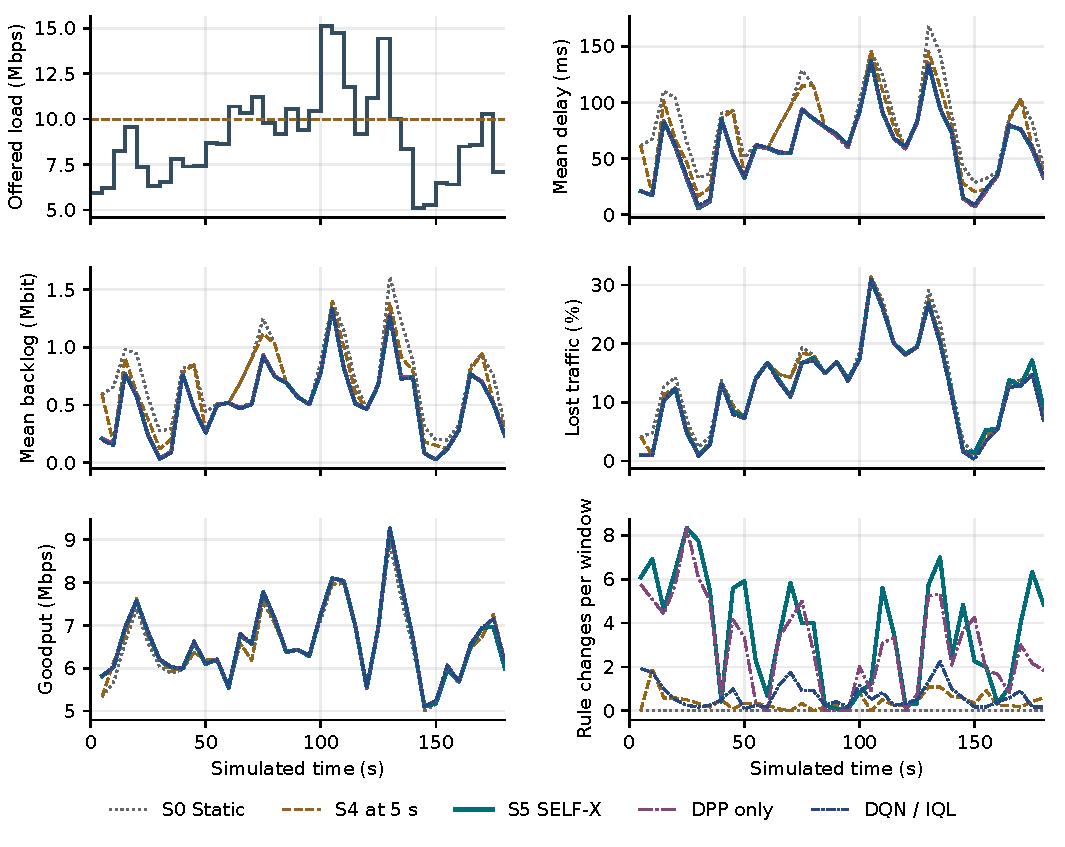
\includegraphics[width=.97\textwidth]{comparison/paper_window_traces.pdf}
\caption{Offered load, delay, mean backlog, traffic loss, goodput, and rule changes in aligned 5~s windows. Each point is the mean across the twelve test traces at that elapsed time. The dashed line in the offered-load panel marks the 10~Mbps capacity of one path. DQN and IQL share one curve because their effective actions coincide.}
\label{fig:windowtraces}
\end{figure*}

\subsection{Performance by workload}
Table~\ref{tab:profiles} shows absolute delay, loss, and goodput for the selected configurations within each synthetic profile. The absolute means complement the paired cadence estimates. Volatile traffic shows the largest delay gap between S4 and S5. In flash crowds, S5 lowers mean delay relative to S4 while losing more traffic. The profile effects are descriptive summaries over four paired traces each.

\begin{table}[t]
\centering
\caption{Mean Outcomes by Synthetic Workload}
\label{tab:profiles}
\footnotesize
\setlength{\tabcolsep}{3.2pt}
\begin{tabular}{@{}llrrr@{}}
\toprule
Workload & Arm & Delay (ms) & Loss (\%) & Mbps\\
\midrule
\ExpandedProfileRows
\bottomrule
\end{tabular}
\end{table}


\section{Discussion and Limitations}
The experiment uses a single two-path fluid model, fixed buffers and guard thresholds, full observation of current demand, one neural training realization per baseline, one small language model, one frozen adapter and assumed model timing. The study does not establish that a small model, as opposed to these prompts and inputs, caused the constant outputs. Exact current-slot prediction is a simulation advantage for DPP and need not hold with sampled or delayed telemetry. Four independent seeds per profile limit precision; results do not generalize to packet timing, physical switches, measured energy, or production traffic. The fixed governor diagnostic is specific to these traces. It does not establish that a fixed schedule would match a language model under new traffic or a different prompt. Further work should vary the topology and workloads, add training seeds, and measure actual end-to-end control delay.

\section{Conclusion}
For the tested workloads, the controlled cadence ablation supports faster analytic actuation. The full stack offers a small delay reduction over the trained neural policies at the cost of higher loss, and the results provide no evidence of a delay benefit over fast DPP alone. The implementation, seed-level data, test configuration, and plotting commands accompany the manuscript.

\section*{Artifact Availability}
The accompanying archive includes the implementation, instructions, twelve paired test seeds, the frozen adapter, the full comparison atlas, and both Deep Review reports. The analysis scripts regenerate the figures, paired comparisons, and workload table from the run manifest.

\IEEEtriggeratref{8}
\bibliographystyle{IEEEtran}
\bibliography{refs}
\end{document}
